\chapter{Implementation}

%The implementation should look at any issues you encountered as you tried to implement your design. During the work, you might have found that elements of your design were unnecessary or overly complex; perhaps third party libraries were available that simplified some of the functions that you intended to implement. If things were easier in some areas, then how did you adapt your project to take account of your findings?
%
%It is more likely that things were more complex than you first thought. In particular, were there any problems or difficulties that you found during implementation that you had to address? Did such problems simply delay you or were they more significant?

%You can conclude this section by reviewing the end of the implementation stage against the planned requirements. 
	
\section{Data Downloading}
\label{sec:imp_data_download}
%discuss data downloader implementation, discussing file name pattern and challenges with that, as well as %difficulties with storage as dataset is large

\section{Data Parsing}
\label{sec:imp_data_parse}
%discuss experimentation with how to extract data from original dataset. discuss change made to format of %parsed data part way through to make it easier to annoate.

\subsection{Name Recognition and Disambiguation}
\label{sec:imp_name_disamb}
%here discuss difficulties in name disambiguation. discuss attempted methods of using NLTKs named entity %thing and the implemented regex solution. Discuss how the regex solution only works because the names are %presented in a predicable pattern, and would not be valid outside of this dataset
Part of the difficulty in parsing the data accurately was ensuring speech spoken by one person was always attributed to that person, even though the references to that person may use multiple versions of their name. In order to correctly attribute speech to the speaker, without duplicating references to them, a method of NLP called "Name Disambiguation" must be employed.

Name Disambiguation is the method of identifying proper names in text, and recognizing when two proper names refer to the same subject or person.\cite{Wacholder} Many difficulties exist for such a task, as names can come in many forms. Proper nouns can often refer to multiple things. \emph{Johnson and Sons} might refer to a business by that name; two people with the surnames \emph{Johnson} and \emph{Sons}; or someone called \emph{Johnson} and their male children. In this example, the context of the sentence the name appears in may provide clues to which it is, but this is not always an option.

Thankfully, this project only needs to be able to recognize the names of the Members of Parliament mentioned in the Hansard Dataset, which displays more structure in the way it names people than normal human speech would.

\begin{figure}[ht]
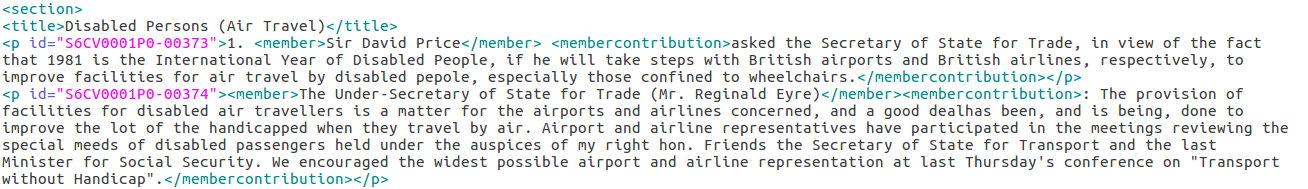
\includegraphics[width=\textwidth]{dataset_name_example}
\caption{An example from the original dataset, showing that names exist only within \emph{member} tags}
\label{fig:dataset_name_example}
\end{figure}

As can be seen in fig.\ref{fig:dataset_name_example}, the names needed for this project are always contained within a \emph{member} tag. They still contain the full job title at times, but this means that the area the project needs to look for a name is well defined. It can be guaranteed that, if a member tag is encountered, it will contain the name of the member.

The first attempted method of extracting the name from the \emph{member} tag was using the \emph{Named Entity Chunker} from NLTK, which is designed to extract the Named Entities from a piece of text and return them in a list. Using this, the name could be extracted, potentially along with other parts of the title (\emph{The Under-Secretary of State for Trade (Mr. Reginald Eyre)} would be returned as a list of two names, \emph{State for Trade} and \emph{Mr. Reginald Eyre}). The thought was that the actual name desired could be chosen from that list by looking for the item that started with an Honorific, such as \emph{Mr.}, \emph{Mrs.} and other such titles. However, the Named Entity Chunker did not work consistently enough for it to be a viable solution for the name extractor, as it often separated the honorific from the name. Due to this, it could not be reliably used to extract the names, because there was no way to recognize, when it returned multiple names, which referred to the actual person, and which was a part of their job title.

The second method attempted, which was the one settled on for the project, was the use of Regular Expressions to search for the expected name format. This method relies on a lot of assumptions about the organization of the original dataset, but appears to be good enough for the current dataset. The assumptions are as follows:
\begin{itemize}
	\item All Names start with an Honorific (Mr, Mrs, Sir etc)
	\item All Names End with a Surname
	\item The first time a person is seen, their full name and job title, if relevant, are presented
\end{itemize}

Following these assumptions, Regular Expressions could be used to find the honorific at the start of the name, then get everything following it until either the end of the text, or a piece of punctuation not commonly used in names, such as a bracket.
\begin{figure}[ht]
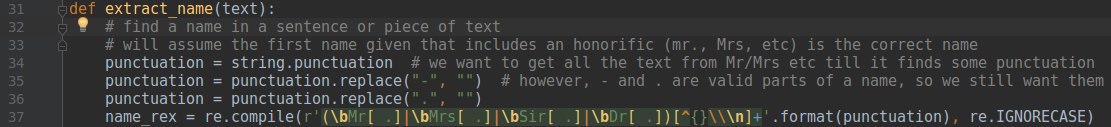
\includegraphics[width=\textwidth]{extract_name_code_example}
\caption{Extract of code from the Name Extractor Method.}
\label{fig:name_extract_code}
\end{figure}

Fig\ref{fig:name_extract_code} shows the regular expression used to extract a name from a piece of text. It searches for an Honorific to start it off, either \emph{Mr}, \emph{Mrs}, \emph{Dr} or \emph{Sir}. Once it find one of these honorifics it gets everything after it that is not a punctuation mark listed, as shown by the \verb|[^{}\\\n]+| part at the end of the regular expression. The \verb|{}| brackets in that part are replaced with the string called \emph{punctuation}, generated by the string package, so that it becomes a list of all punctuation possible, including new line characters.  

\subsection{Name Matching}
\label{sec:imp_name_match}
Once names can be reliably extracted from the source text, a method of comparing two names to see if they referred to the same person had to be developed. This becomes a very complicated issue, simplified only slightly by the assumptions mentioned previously.

\begin{table}[ht!]
\centering
\begin{tabular}{|c c c|}
Name One & Name Two & Same Person? \\
\hline
Mr. Adam Neaves  & Mr. Adam Neaves & True \\
Mr. A. Neaves    & Mr. Adam Neaves & True \\
Dr. Adam Neaves  & Mr. Adam Neaves & False, wrong Honorific \\
Mr. B. Neaves    & Mr. Adam Neaves & False, wrong First Name \\
Adam Neaves      & Mr. Adam Neaves & True, despite missing honorific \\
Mr. A. B. Neaves & Mr. Adam Neaves & True, though slightly ambiguous \\
Mr. A. B. Neaves & Mr. Neaves      & True, though again ambiguous    \\
\end{tabular}
\caption{Table showing the different ways names might or might not refer to the same person}
\label{tbl:name_match}
\end{table}

For instance, as shown in table \ref{tbl:name_match}, first names might be shortened to just an initial, or even fully removed. Honorifics are not guaranteed to be present, but are very important if they are, as two different names may differ from only that.

The implemented algorithm for this project follows the same assumptions mentioned in section \ref{sec:imp_name_disamb}, and is designed to allow for some false negatives (wherein two names that \emph{do} refer to the same person might not appear as the same person) to avoid any false positives at all, as speech accidentally attributed to the wrong person would be worse than accidentally having duplicate references to a person. The basic algorithm implemented is as follows:
\begin{lstlisting}
if BOTH NAMES ARE EXACTLY THE SAME
	return True
SPLIT BOTH NAMES INTO COMPONENT WORDS
for EACH NAME
	if NAME CONTAINS 3 WORDS
		FIRST WORD IS HONORIFIC
		SECOND WORD IS FORENAME
		THIRD WORD IS SURNAME
	else
		FIRST WORD IS HONORIFIC
		LAST WORD IS SURNAME
		IGNORE ANYTHING ELSE
if FORENAME ONE and FORENAME TWO BOTH EXIST
	FORNAME_MATCH = FORNAME ONE == FORNAME TWO
else
	FORNAME_MATCH = True
SURNAME_MATCH = SURNAME ONE == SURNAME TWO
HONORIFIC_MATCH = HONORIFC ONE == HONORIFIC TWO

if SURNAME_MATCH, HONORIFIC_MATCH and FORENAME_MATCH ARE True
	return true
else return False
\end{lstlisting}